\documentclass{article}

% ------------ packages -------------

\usepackage[utf8]{inputenc}
\usepackage[OT1]{fontenc}
\usepackage{graphicx}
\usepackage[english]{babel}

\usepackage{amsmath}
\usepackage{amsfonts}
\usepackage{amssymb}
\usepackage{amsthm}
\usepackage{bm}

\usepackage[usenames,dvipsnames]{xcolor}
\usepackage{booktabs}
\usepackage{tikz}
\usepackage{sidecap}

\usepackage{url}
\usepackage[bookmarks]{hyperref}

%\usetikzlibrary{shapes.misc,fit}
\usetikzlibrary{%
   arrows,%
   calc,%
   fit,%
   patterns,%
   plotmarks,%
   shapes.geometric,%
   shapes.misc,%
   shapes.symbols,%
   shapes.arrows,%
   shapes.callouts,%
   shapes.multipart,%
   shapes.gates.logic.US,%
   shapes.gates.logic.IEC,%
   er,%
   automata,%
   backgrounds,%
   chains,%
   topaths,%
   trees,%
   petri,%
   mindmap,%
   matrix,%
   calendar,%
   folding,%
   fadings,%
   through,%
   patterns,%
   positioning,%
   scopes,%
   decorations.fractals,%
   decorations.shapes,%
   decorations.text,%
   decorations.pathmorphing,%
   decorations.pathreplacing,%
   decorations.footprints,%
   decorations.markings,%
   shadows}

% ------------ custom defs -------------

\newcommand{\reals}{\mathbb{R}}
\newcommand{\posreals}{\reals_{>0}}
\newcommand{\posrealszero}{\reals_{\ge 0}}
\newcommand{\naturals}{\mathbb{N}}

\newcommand{\dd}{\,\mathrm{d}}

\newcommand{\mbf}[1]{\mathbf{#1}}
\newcommand{\bs}[1]{\boldsymbol{#1}}
\renewcommand{\vec}[1]{{\bm#1}}

\newcommand{\uz}{^{(0)}} % upper zero
\newcommand{\un}{^{(n)}} % upper n
\newcommand{\ui}{^{(i)}} % upper i

\newcommand{\ul}[1]{\underline{#1}}
\newcommand{\ol}[1]{\overline{#1}}

\newcommand{\Tsys}{T_\text{sys}}

\newcommand{\Rsys}{R_\text{sys}}
\newcommand{\lRsys}{\ul{R}_\text{sys}}
\newcommand{\uRsys}{\ol{R}_\text{sys}}

\newcommand{\fsys}{f_\text{sys}}
\newcommand{\Fsys}{F_\text{sys}}
\newcommand{\lFsys}{\ul{F}_\text{sys}}
\newcommand{\uFsys}{\ol{F}_\text{sys}}

\newcommand{\lgt}{\ul{g}}
\newcommand{\ugt}{\ol{g}}

\newcommand{\E}{\operatorname{E}}
\newcommand{\V}{\operatorname{Var}}
\newcommand{\wei}{\operatorname{Wei}} % Weibull Distribution
\newcommand{\ig}{\operatorname{IG}}   % Inverse Gamma Distribution

\newcommand{\El}{\ul{\operatorname{E}}}
\newcommand{\Eu}{\ol{\operatorname{E}}}

\def\yz{y\uz}
\def\yn{y\un}
%\def\yi{y\ui}
\newcommand{\yfun}[1]{y^{({#1})}}
\newcommand{\yfunl}[1]{\ul{y}^{({#1})}}
\newcommand{\yfunu}[1]{\ol{y}^{({#1})}}

\def\ykz{y\uz_k}
\def\ykn{y\un_k}

\def\yzl{\ul{y}\uz}
\def\yzu{\ol{y}\uz}
\def\ynl{\ul{y}\un}
\def\ynu{\ol{y}\un}
\def\yil{\ul{y}\ui}
\def\yiu{\ol{y}\ui}

\def\ykzl{\ul{y}\uz_k}
\def\ykzu{\ol{y}\uz_k}
\def\yknl{\ul{y}\un_k}
\def\yknu{\ol{y}\un_k}

\newcommand{\ykzfun}[1]{y\uz_{#1}}
\newcommand{\ykzlfun}[1]{\ul{y}\uz_{#1}}
\newcommand{\ykzufun}[1]{\ol{y}\uz_{#1}}


\def\nz{n\uz}
\def\nn{n\un}
%\def\ni{n\ui}
\newcommand{\nfun}[1]{n^{({#1})}}
\newcommand{\nfunl}[1]{\ul{n}^{({#1})}}
\newcommand{\nfunu}[1]{\ol{n}^{({#1})}}

\def\nkz{n\uz_k}
\def\nkn{n\un_k}
\newcommand{\nkzfun}[1]{n\uz_{#1}}
\newcommand{\nkzlfun}[1]{\ul{n}\uz_{#1}}
\newcommand{\nkzufun}[1]{\ol{n}\uz_{#1}}

\def\nzl{\ul{n}\uz}
\def\nzu{\ol{n}\uz}
\def\nnl{\ul{n}\un}
\def\nnu{\ol{n}\un}
\def\nil{\ul{n}\ui}
\def\niu{\ol{n}\ui}

\def\nkzl{\ul{n}\uz_k}
\def\nkzu{\ol{n}\uz_k}
\def\nknl{\ul{n}\un_k}
\def\nknu{\ol{n}\un_k}

\def\yknow{y_k^{(\tnow)}}
\def\nknow{n_k^{(\tnow)}}

\newcommand{\nk}{n_k}
\newcommand{\nkp}{n_k'}
\newcommand{\yk}{y_k}
\newcommand{\ykp}{y_k'}

\def\taut{\tau(\vec{t})}
\def\ttau{\tilde{\tau}}
\def\ttaut{\ttau(\vec{t})}
\def\tautk{\tau(\vec{t}_k)}

\def\MZ{\mathcal{M}\uz}
\def\MN{\mathcal{M}\un}

\def\MkZ{\mathcal{M}\uz_k}
\def\MkN{\mathcal{M}\un_k}

\def\PkZ{\Pi\uz_k}
\def\PkN{\Pi\un_k}
\newcommand{\PZi}[1]{\Pi\uz_{#1}}

\def\tnow{t_\text{now}}
\def\tpnow{t^+_\text{now}}

\newcommand{\Rsysnow}{R^{(t_\text{now})}_\text{sys}}
\newcommand{\Tsysnow}{T^{(t_\text{now})}_\text{sys}}
\newcommand{\tsysnow}{t^{(t_\text{now})}_\text{sys}}
\newcommand{\fsysnow}{f^{(t_\text{now})}_\text{sys}}
\def\eknow{e_k^{(\tnow)}}
\def\cknow{c_k^{(\tnow)}}
\def\vectknow{\vec{t}_k^{(\tnow)}}
\def\Phinow{\Phi^{(\tnow)}}
\newcommand{\gnow}{g^{(\tnow)}}
\newcommand{\tausnow}{\tau_*^{(\tnow)}}
\newcommand{\tprep}{\tau_{\text{prep}}}
\newcommand{\tthresh}{\tau_{\text{thresh}}}
\newcommand{\tstarnow}{t_*^{(\tnow)}}
\newcommand{\gstarnow}{g_*^{(\tnow)}}
\newcommand{\gtotalnow}{g_\text{total}^{(\tnow)}}
\newcommand{\esys}{e_\text{sys}}
\newcommand{\mrsys}{\bar{r}_\text{sys}}

\begin{document}
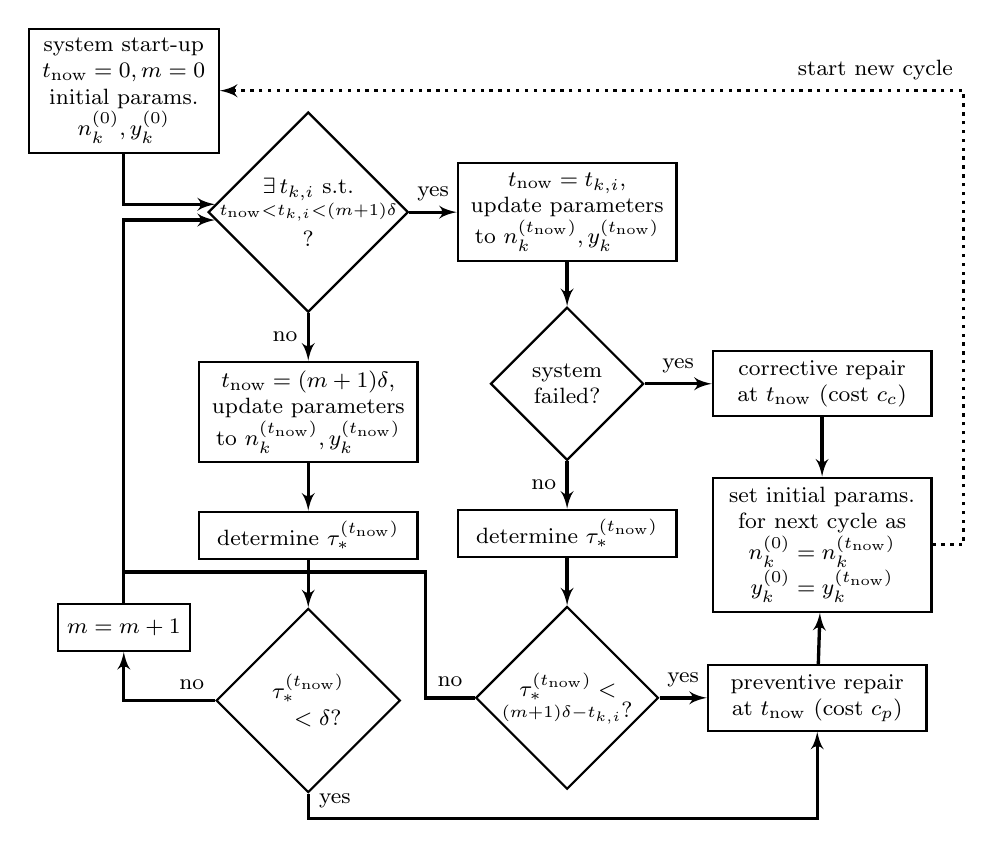
\begin{tikzpicture}
[node distance=6mm,
 font=\footnotesize,
 box/.style={draw, rectangle, thick, minimum height=6mm, minimum width=15mm},
 box2/.style={draw, rectangle, thick, minimum height=6mm, minimum width=28mm, rounded corners=2mm},
 dec/.style={draw, shape=diamond, thick, minimum height=4mm, minimum width=4mm},
 pfeil/.style={-latex', very thick}]
\node (startup) [box] {\parbox{18ex}{\centering system start-up\\ $\tnow = 0, m= 0$\\ initial params.\\ $\nkz, \ykz$}};
\node (mincrem) [box, below=57mm of startup] {$m = m + 1$};
\node (cptfail) [dec, below right=9mm and 17mm] {\parbox{10ex}{\centering $\exists\, t_{k,i}$ s.t.\\ \rule{0ex}{2ex} \\ ?}};
%$(m-1)\delta$\\ $ < t_{k,i} < $\\ $m\delta$}};
\node at (cptfail) {$\scriptstyle \tnow < t_{k,i} < (m+1)\delta$};
%\coordinate (mcoord) at ($(startup) * (0, -2)$) {};
\node (nfltnow) [box, below=of cptfail] {\parbox{21ex}{\centering $\tnow = (m + 1)\delta$,\\ update parameters\\ to $\nknow, \yknow$}};
\node (yfltnow) [box, right=of cptfail] {\parbox{21ex}{\centering $\tnow = t_{k,i}$,\\ update parameters\\ to $\nknow, \yknow$}};
\node (sysfail) [dec, below=5.6mm of yfltnow] {\parbox{8ex}{\centering system\\ failed?}};
\node (tausmde) [box, below=of nfltnow] {\parbox{21ex}{\centering determine $\tausnow$}};
\node (taustki) [box, below=of sysfail] {\parbox{21ex}{\centering determine $\tausnow$}};
\node (tausdel) [dec, below=of tausmde] {\parbox{10ex}{\centering $\tausnow$\\ \rule{2ex}{0ex}$< \delta$?}};
\node (taudtki) [dec, below=of taustki] {\parbox{10ex}{$\tausnow <$\\ \phantom{?}}};
\node at ($(taudtki) + (0,-2mm)$) {$\scriptstyle (m + 1) \delta - t_{k,i}$?};
\node (corrmnt) [box, right=8.5mm of sysfail] {\parbox{21ex}{\centering corrective repair\\ at $\tnow$ (cost $c_c$)}};
\node (prevmnt) [box, right=of taudtki] {\parbox{21ex}{\centering preventive repair\\ at $\tnow$ (cost $c_p$)}};
\node (updatep) [box, below=7.5mm of corrmnt] {\parbox{21ex}{\centering set initial params.\\ for next cycle as\\ $\nkz = \nknow$\\ $\ykz = \yknow$}};
%\coordinate (nocoord) at ($(taudtki) + (-1.8,-1.3)$) {};
\coordinate (nocoord) at ($(taudtki) + (-1.8, 1.6)$) {};
\coordinate (yscoord) at ($(tausdel) + ( 0  ,-1.5)$) {};
\coordinate (nxtcoor) at ($(updatep) + ( 1.8, 0  )$) {};
\draw[pfeil] (startup) |- ($(cptfail.west) + (0.1, 0.1)$);
\draw[pfeil] (mincrem) |- ($(cptfail.west) + (0.1,-0.1)$);
\draw[pfeil] (cptfail) -- (nfltnow) node[midway, left] {no};
\draw[pfeil] (cptfail) -- (yfltnow) node[midway, above] {yes};
\draw[pfeil] (yfltnow) -- (sysfail);
\draw[pfeil] (nfltnow) -- (tausmde);
\draw[pfeil] (sysfail) -- (taustki) node[midway, left] {no};
\draw[pfeil] (sysfail) -- (corrmnt) node[midway, above] {yes};
\draw[pfeil] (tausmde) -- (tausdel);
\draw[pfeil] (taustki) -- (taudtki);
\draw[pfeil] (tausdel) -| (mincrem) node[at start, above left] {no};
\draw[very thick] (taudtki) -| (nocoord) node[near start, above] {no} -| (mincrem);
\draw[pfeil] (taudtki) -- (prevmnt) node[midway, above] {yes};
\draw[pfeil] (tausdel) -- (yscoord) -| (prevmnt) node[at start, above right] {yes};
\draw[pfeil] (prevmnt) -- (updatep);
\draw[pfeil] (corrmnt) -- (updatep);
\draw[pfeil, dotted] (updatep) -- (nxtcoor) |- (startup) node[midway, above left] {start new cycle};
%
%\node (startup) [box]                       {\parbox{20ex}{\centering system start-up\\ (all comp.\ new)}};
%\node (sysfail) [box, right=of startup]     {system failed?};
%\node (tauchck) [box, below=6mm of sysfail] {$\tausnow < \delta$?};
%\node (gotonxt) [box, below=6mm of tauchck] {\parbox{17ex}{\centering continue to\\ $\tnow = (m+1)\delta$}};
%\draw [thick, dashed, rounded corners=2mm] ($(gotonxt.south east) + (2mm,-1mm)$) rectangle ($(sysfail.north west) + (-5mm,1mm)$) node[above left=0mm and -33mm] {each $\tnow = m \delta, m \in \naturals_0$};
%\node [above left=0mm and -8mm of startup] {$t=0$};
%\node (correct) [box, right=of sysfail, minimum width=18mm] {\parbox{14ex}{\centering corrective\\ maintenance\\ (cost $c_c$)}};
%\node (prevent) [box, right=of tauchck, minimum width=18mm] {\parbox{14ex}{\centering preventive\\ maintenance\\ (cost $c_p$)}};
%\node (update) [box, below right=10mm and -4mm of prevent, minimum width=10mm] {\parbox{12ex}{\centering update parameters}};
%\draw[pfeil] (startup) -- (sysfail);
%\draw[pfeil] (sysfail) -- (tauchck) node[midway, right] {no};
%\draw[pfeil] (tauchck) -- (gotonxt) node[midway, right] {no};
%\draw[very thick] (gotonxt.west) -| ($(sysfail.west) + (-3mm,0mm)$);
%\draw[pfeil] (sysfail) -- (correct) node[midway, above] {yes};
%\draw[pfeil] (tauchck) -- (prevent) node[midway, above] {yes};
%\draw[pfeil] (correct) -| (update);
%\draw[pfeil] (prevent) -| (update);
%\draw[pfeil, dotted] (update) -| (startup) node[midway, below right] {start new cycle};
\end{tikzpicture}
\end{document}
